
\documentclass{beamer}

\mode<presentation> {
\usetheme{Warsaw}
}

\usepackage{graphicx}
\usepackage{booktabs}
\usepackage{listings}
\usepackage{color}
\usepackage{hyperref}
\usepackage[lofdepth,lotdepth]{subfig}
\usepackage{hyperref}
\usepackage{fontawesome}

\definecolor{codegreen}{rgb}{0,0.6,0}
\definecolor{codegray}{rgb}{0.5,0.5,0.5}
\definecolor{codepurple}{rgb}{0.58,0,0.82}
\definecolor{backcolour}{rgb}{0.95,0.95,0.92}

\lstdefinestyle{mystyle}{
    backgroundcolor=\color{backcolour},   
    commentstyle=\color{codegreen},
    keywordstyle=\color{magenta},
    numberstyle=\tiny\color{codegray},
    stringstyle=\color{codepurple},
    %basicstyle=\footnotesize,
    basicstyle=\scriptsize\ttfamily,
    breakatwhitespace=false,         
    breaklines=true,                 
    captionpos=b,                    
    keepspaces=true,                 
    numbers=left,                    
    numbersep=5pt,                  
    showspaces=false,                
    showstringspaces=false,
    showtabs=false,                  
    tabsize=2,
    language=bash
}
 
\lstset{style=mystyle}

% \newcommand{\SubItem}[1]{
%     {\setlength\itemindent{15pt} \item[-] #1}
% }

%------------
%	TITLE PAGE
%------------

\title[Version control, Git and GitHub]{Introduction to Git} 
\author{Criscely Luj\'{a}n}
\institute[Universit\'{e} Paris-Sud, UMR MARBEC]  
{Universit\'{e} Paris-Sud, UMR MARBEC \\ 
\medskip
\textit{criscely.lujan@ird.fr}}
\date{April 11, 2019}

\begin{document}

%------------
\begin{frame}
\titlepage 
\begin{center}

\includegraphics[height=1.5cm]{img/logo_psud.jpg}
\hspace{1em}

\includegraphics[height=1.5cm]{img/logo_marbec.png}
\hspace{1em}

\includegraphics[height=1.5cm]{img/logo_ird.png}
\end{center}
\end{frame}


\begin{frame}
\frametitle{Version control}

Also known as \textbf{revision control} or \textbf{source control}. \hfill \break

... ``\textit{is the management of changes:}

\begin{itemize}
    \item \textit{documents
    \item computer programs
    \item large web sites
    \item other collections of information ... }''
\end{itemize}
\end{frame}


\begin{frame}
\frametitle{Why is important version control?}
\begin{center}

\includegraphics[scale=0.29]{img/phd_comics.png}
\end{center}
\end{frame}


\begin{frame}
\frametitle{Why is important version control?}
\begin{itemize}
    \item Storing \textbf{version} (properly). \hfill \break
    \item \textbf{Restoring} previous versions. \hfill \break
    \item \textbf{Collaborations} (networking). \hfill \break
    \item Save \textbf{time}. \hfill \break
\end{itemize}
\end{frame}


\begin{frame}
\frametitle{Version control software}
\begin{center}
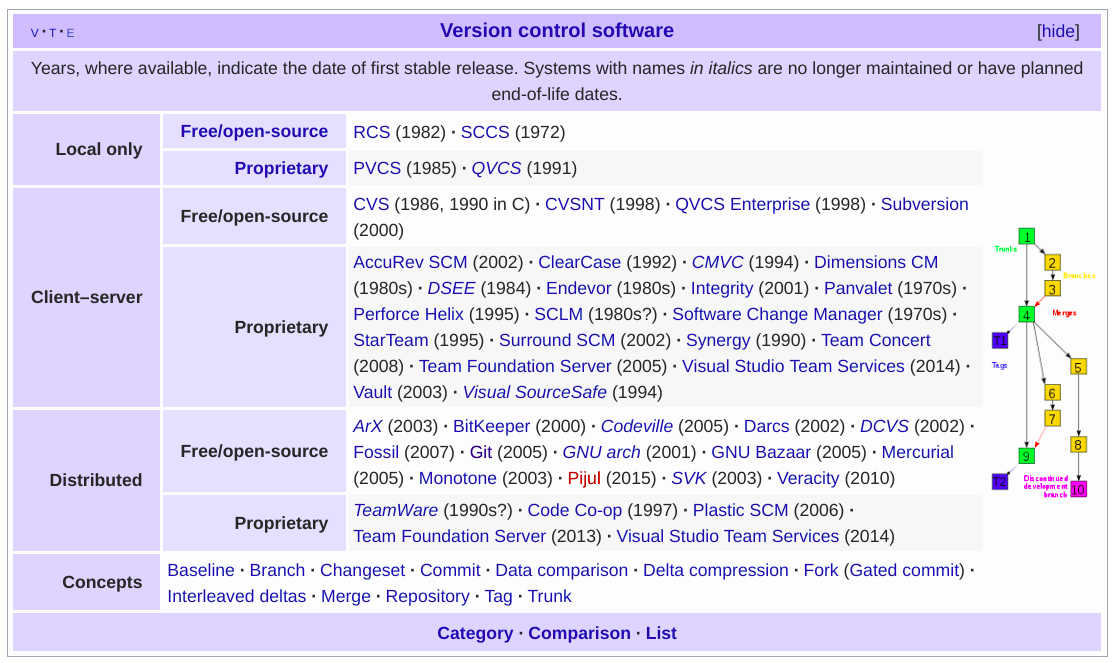
\includegraphics[scale=0.29]{img/controlVersion.png}
\end{center}
\end{frame}


\begin{frame}
\frametitle{What is Git?}

\textbf{Git} is a distributed version control system for tracking changes in source code during the development of software.

 \hfill \break

\begin{center}

\includegraphics[scale=0.07]{img/git_logo.png}
\end{center}
\end{frame}


\begin{frame}
\frametitle{Why use Git?}
\begin{itemize}
    \item \textbf{Popular and successful}
      \begin{itemize}
      \item[$-$]{Active development}
      \item[$-$]{Fast}
      \hfill \break
      \end{itemize}
      
    \item \textbf{Distributed}
      \begin{itemize}
      \item[$-$]{Work online and offline}
      \item[$-$]{Collaborate with large groups}
      \hfill \break
      \end{itemize}
    
    \item \textbf{Tracks any type of file}
      \begin{itemize}
      \item[$-$]{Works best with text}
      \hfill \break
      \end{itemize}
    
    \item \textbf{Branching}
      \begin{itemize}
      \item[$-$]{Smarter merges}
      \end{itemize}
\end{itemize}
\end{frame}


\begin{frame}
\frametitle{What is GitHub Inc.?}

\begin{center}
\textbf{GitHub} is a web-based hosting service for version control using \textbf{Git}.
\end{center}

\begin{center}

\includegraphics[scale=0.2]{img/github_logos.png}
\end{center}
\end{frame}


\begin{frame}
\frametitle{GitHub Inc.}
\begin{itemize}
    \item Access to the control and collaboration features for every \textbf{project}. \hfill \break
    \item Work with public and private \textbf{repositories}. \hfill \break
    \item Develop a \textbf{networking}. \hfill \break
    \item \textbf{Plans} for enterprise, teams, pro and free accounts. \hfill \break
    \item Is the \textbf{largest} host of source code in the world! \emph{(28 million users, 57 million repositories (28 million public) - June 2018)}.
\end{itemize}
\end{frame}


\begin{frame}
\frametitle{Register a GitHub account}
\begin{itemize}
    \item Register an account with \href{https://github.com/}{\faStar GitHub} is free! \hfill \break
    \item Free private repositories
          \begin{itemize}
          \item[$-$] Sudents, faculty, and educational / research staff: \href{https://education.github.com/}{\faStar GitHub Education}.
          \item[$-$] Official nonprofit organizations and charities: \href{https://github.com/nonprofit}{\faStar GitHub for Good}.
          \hfill \break
          \end{itemize}
    \item Pay for private repositories
          \begin{itemize}
          \item[$-$] Individual cost is 7 dolars per month: \href{https://github.com/pricing}{\faStar GitHub Pricing}.
          \end{itemize}

\end{itemize}
\end{frame}


\begin{frame}
\frametitle{Git clients}

Git and Git client \textbf{are not} the same! Like R and RStudio is not the same thing!
\hfill \break

Git client:
\begin{itemize}
    \item IDE (Integrated development environment)!
    \item Make the experience more pleasant providing a richer visual representation.
\end{itemize}

\hfill 

Some Git clients:
\begin{itemize}
    \item \href{https://www.sourcetreeapp.com/}{\faStar SourceTreen} 
    \item \href{https://www.gitkraken.com/}{\faStar GitKraken}
    \item \href{https://gitup.co/}{\faStar GitUp} 
    \item \href{https://www.syntevo.com/smartgit/}{\faStar SmartGit} 
    \item \href{https://git-cola.github.io/}{\faStar git-cola} 
    \item ... others... 
    \item \textbf{RStudio} 
\end{itemize}
\end{frame}



\end{document}